\documentclass[9pt]{beamer}
\usepackage{graphicx}
\usepackage{amsmath}
\usepackage{amssymb}
\usepackage[T1]{fontenc}
%\usepackage{movie15}
\usepackage{subfigure}

%\usetheme{default}
%\usecolortheme{dolphin}
\usepackage{pgf}
\usepackage{beamerthemesplit}

\definecolor{kugreen}{RGB}{50,93,61}
\definecolor{kugreenlys}{RGB}{132,158,139}
\definecolor{kugreenlyslys}{RGB}{173,190,177}
\definecolor{kugreenlyslyslys}{RGB}{214,223,216}
\definecolor{mygreen}{rgb}{0.4,0.4,0.7}
\setbeamercovered{transparent}
\mode<presentation>
\usetheme{CambridgeUS}
%\setbeamertemplate{footline}[frame number]
 
\usecolortheme[]{seahorse}
\useinnertheme{circles}
\usefonttheme[onlymath]{serif}
\setbeamercovered{transparent}
\setbeamertemplate{blocks}[rounded][shadow=true]

\setbeamerfont{frametitle}{size={\fontsize{12}{12}}}

\newcommand{\rf}{\textbf{R}}
\newcommand{\p}{\partial}
\newcommand{\rh}{\hat{r}}
\newcommand{\lb}{\left(}
\newcommand{\rb}{\right)}

\title[SRG Quantum Dots]{SRG applied to Quantum Dots - what I have done so far}
\author{Sarah Reimann}
\institute[UiO]{Department of Physics, University of Oslo, Norway}

\begin{document}


\begin{frame}
\titlepage
\end{frame}

%\begin{frame}
%\frametitle{Outline}
%\tableofcontents
%\end{frame}

\AtBeginSubsection[]
{
 \begin{frame}<beamer>
\frametitle{Outline}
\tableofcontents[currentsection, currentsubsection]
 \end{frame}
}

\begin{frame}
\frametitle{Aim of the thesis}
\begin{itemize}
\item Study the ground state of closed-shell systems of quantum dots in two dimensions
\item Method: Similarity renormalization group (SRG) method 
\item Use of the same methodology discussed in the paper 'Similarity renormalization group for nucleon-nucleon interactions' by S.K.Bogner et al.
\end{itemize}
\end{frame}


\section{Implementation}
\begin{frame}
\frametitle{Implemented equations}
The Hamiltonian:
\[
H = T_{\rm rel} + V
\]
\begin{center}
$T_{\rm rel}$: relative kinetic energy, $V$: interaction part
\end{center}
Flow of the Hamiltonian:
\[
\frac{d H_s}{ds} = \left[\eta_s, H_s \right]
\]
Choice of generator:
\[
\eta_s = \left[T_{\rm rel}, H_s\right] = \left[T_{\rm rel}, V_s\right]
\]

Only interaction part $V$ dependent on flow parameter $s$!\\

\textbf{Chosen basis}: Harmonic oscillator basis
\[
T_{\rm rel} =
 \left( \begin{array}{cccc}
T_0 & 0 & \dots & 0 \\
0 & T_1 & \dots & 0 \\
\dots & \dots & \dots & \dots \\
0 & 0 & \dots & T_n \end{array} \right)
\]
with $T_i = \sum\limits_{i=1}^N \epsilon_i = \sum\limits_{i=1}^N \hbar\omega (2n_i + |m_i| +1)$,
 $N$ - number of particles.
\end{frame}

\begin{frame}
\frametitle{Implemented equations}
With this choice of $T_{\rm rel}$:
\[
 \eta_{ij}(s) = \left( \epsilon_i - \epsilon_j \right) V_{ij}(s).
\]
The flow of the matrix elements is then given by 
\begin{equation}
\frac{d H_{ij}}{ds }= \frac{d V_{ij}}{ds } = -(\epsilon_i - \epsilon_j)^2 V_{ij}(s) + \sum\limits_k \left(\epsilon_i + \epsilon_j -2 \epsilon_k \right) V_{ik}(s) V_{kj}(s).
\label{eq:flow}
\end{equation}



\end{frame}

\begin{frame}
\frametitle{General procedure}
\begin{enumerate}[1)]
\item Specify the number of particles/shells.
\item Set up the \textbf{basis states in M-scheme}, using binary representation. Since I am interested in the ground state, I take only those states where $M = M_s = 0$ ($H$ is block diagonal).
\item Set up of the \textbf{initial Hamiltonian matrix}, dimension $n\times n$. Interaction matrix elements are computed using the code of S. Kvaal.
\item \textbf{Solve the system} of $n(n+1)/2$ coupled first-order differential equations using the SRG method (since the Hamiltonian is symmetric, I only consider the upper triangular part)
\end{enumerate}
\end{frame}

\begin{frame}
\frametitle{Details - SRG method}
\begin{itemize}
\item ODE solver: Algorithm by Lawrence Shampine, Marilyn Gordon. C++ version found on netlib.org
\item Derivative function
\begin{enumerate}[-]
\item Flow parameter $s$, related to $\lambda$ by:
$ \lambda = s^{-1/2} $
\item In terms of $\lambda$, this means for the flow
\[
\frac{dV_{ij}(s(\lambda))}{ds} = -\frac{2}{\lambda^3}\frac{dV_{ij}(\lambda)}{d\lambda}
\]
\item Alltogether: Each time the derivative-function is called, compute for each interaction element $V_{ij}(s)$
\[
\frac{d V_{ij}(s(\lambda))}{ds} = -\frac{2}{\lambda^3}\left\lbrace-(\epsilon_i - \epsilon_j)^2 V_{ij}(\lambda) + \sum\limits_k \left(\epsilon_i + \epsilon_j -2 \epsilon_k \right) V_{ik}(\lambda) V_{kj}(\lambda)\right\rbrace.
\]
\end{enumerate}
\end{itemize}

\end{frame}

\section{First results}
\begin{frame}
\frametitle{Some results for the ground state energy}
\begin{table}
\begin{center}
\small
\tabcolsep=0.09cm
\begin{tabular}{|c| c c| c c| c c |}
\hline\hline
 & \multicolumn{2}{|c|}{R = 3} & \multicolumn{2}{|c|}{R = 4} & \multicolumn{2}{|c|}{R = 5}\\
 N & SRG&FCI & SRG &FCI & SRG &  FCI\\
 \hline
 2 & 3.038604576&3.038604576&  3.025230582& 3.025230582& 3.01760623 &3.01760623 \\
 6 & 21.42058830& 21.42058830 &  20.41582765&  20.41582765 & \dots & \dots\\
 12 & -&- &  70.3125021{\color{red}{9}} &70.3125021{\color{red}{8}} & \dots & \dots \\
 \hline\hline
\end{tabular}
\end{center}
\caption{$E_0$ in units of $\hbar\omega = 2.84$ meV. For $N = 2$ particles I performed calculations up to $R = 9$ shells and obtained always exactly the same result as with exact diagonalization.}
\end{table}

\textbf{Pro:} SRG converges to the {\color{red}{exact}} ground state energy for all studied systems.\\
\textbf{Con:} The {\color{red}{required timed}} is exceedingly large, much larger than exact diagonalization, therefore until now just very small systems in reasonable times possible (see next slides)
\end{frame}

\begin{frame}
\frametitle{Pro: convergence of $E_0$! }
\begin{figure}
\subfigure[$N = 2, R = 3$]{\includegraphics[scale=0.18]{../Code/Outputs/HOBasis/2_3/energy.pdf}}
\subfigure[$N = 2, R = 4$]{\includegraphics[scale=0.18]{../Code/Outputs/HOBasis/2_4/energy.pdf}}
\subfigure[$N = 2, R = 5$]{\includegraphics[scale=0.18]{../Code/Outputs/HOBasis/2_5/energy.pdf}}
\subfigure[$N = 6, R = 3$]{\includegraphics[scale=0.18]{../Code/Outputs/HOBasis/6_3/energy.pdf}}
\subfigure[$N = 6, R = 4$]{\includegraphics[scale=0.18]{../Code/Outputs/HOBasis/6_4/energy.pdf}}
\subfigure[$N = 12, R = 4$]{\includegraphics[scale=0.18]{../Code/Outputs/HOBasis/12_4/energy.pdf}}
\end{figure}
\end{frame}

\begin{frame}
\frametitle{Pro: Suppression of off-diagonal matrix elements!}
\begin{figure}
\subfigure{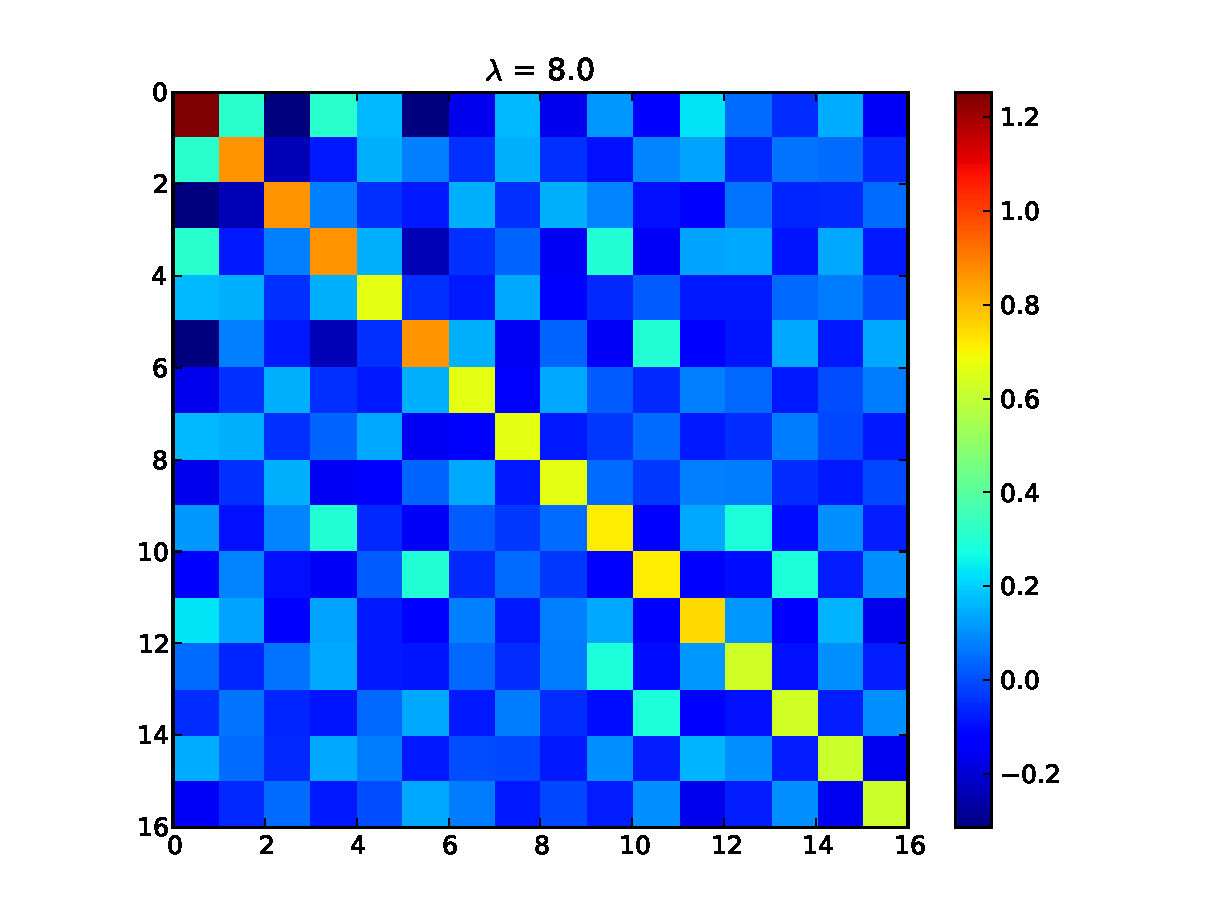
\includegraphics[scale=0.19]{../Code/Outputs/HOBasis/2_4/Hstart.pdf}}
\subfigure{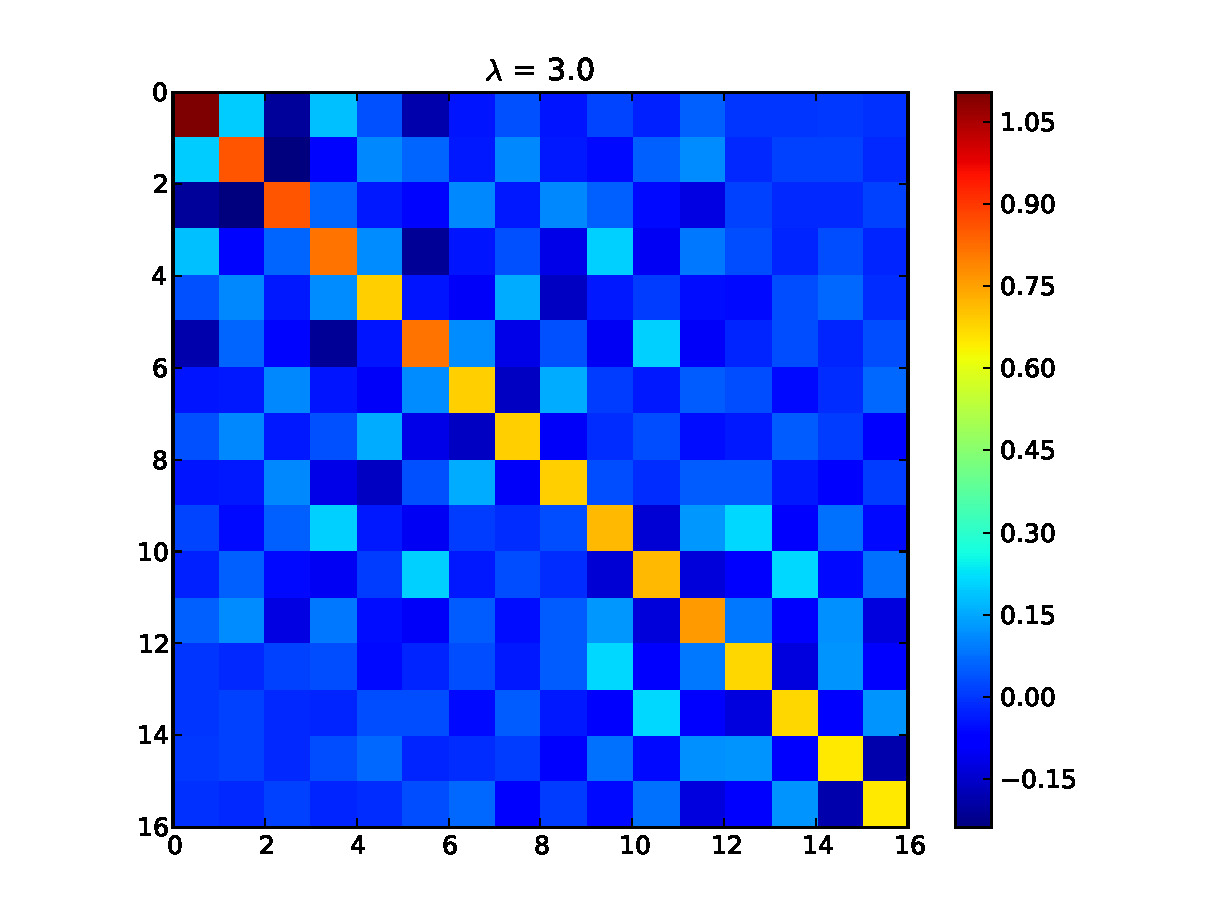
\includegraphics[scale=0.19]{../Code/Outputs/HOBasis/2_4/H3.pdf}}
\subfigure{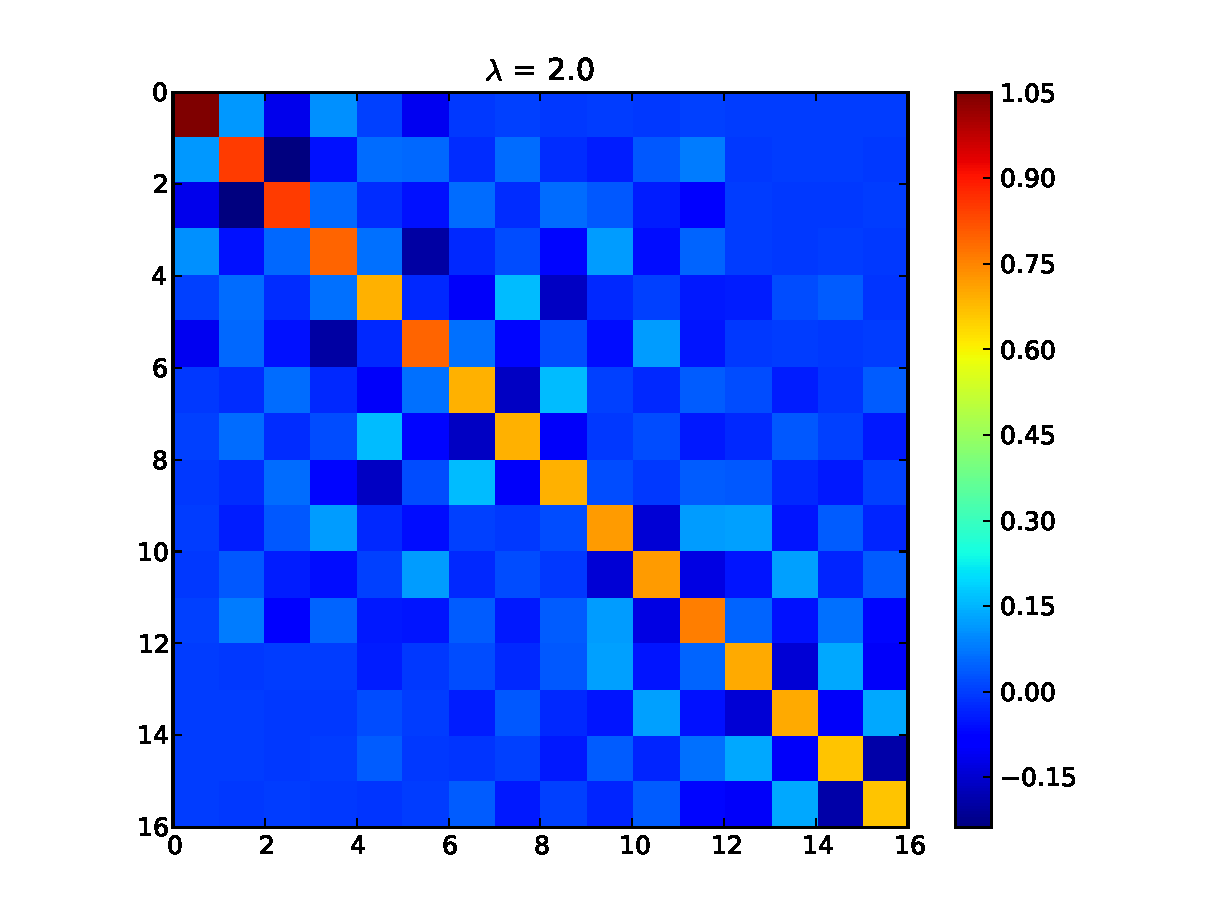
\includegraphics[scale=0.19]{../Code/Outputs/HOBasis/2_4/H2.pdf}}
\subfigure{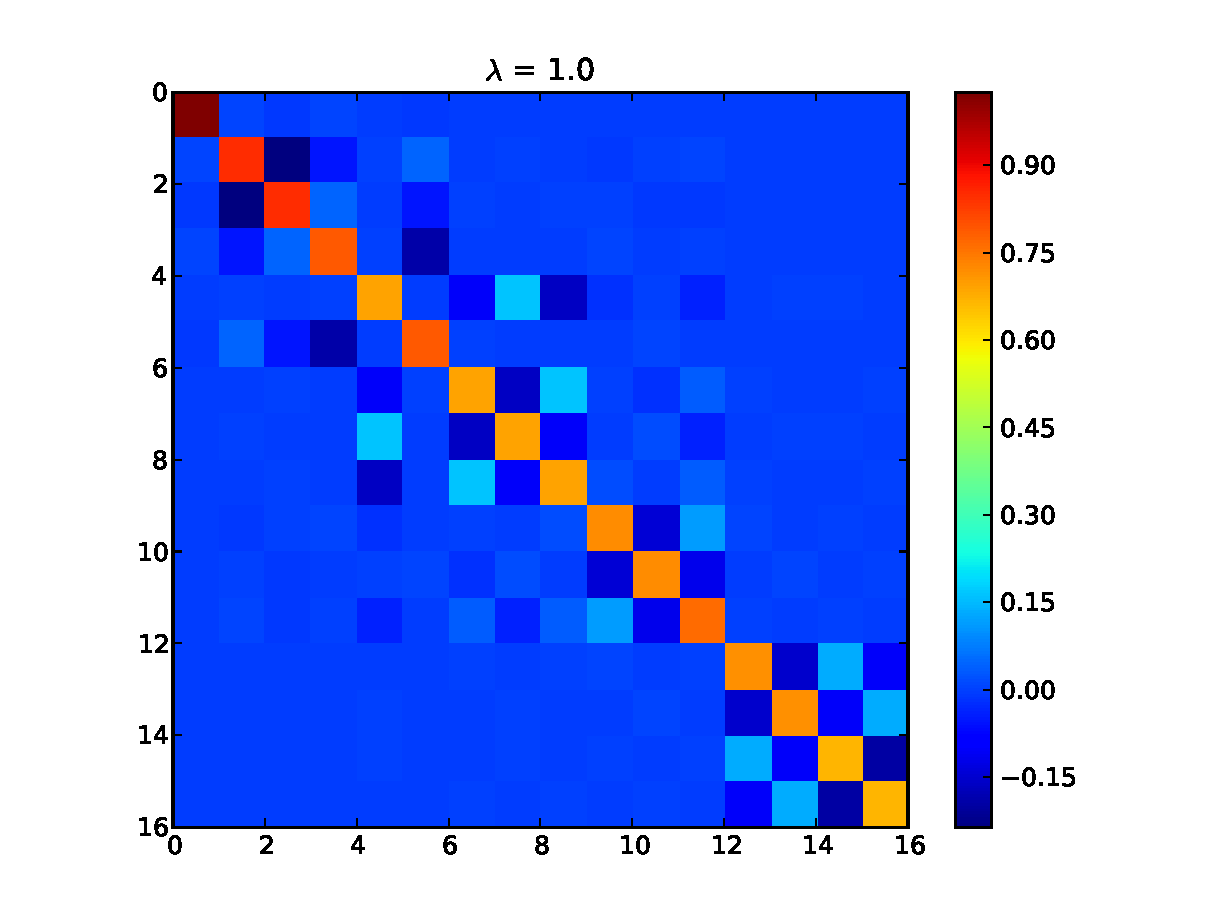
\includegraphics[scale=0.19]{../Code/Outputs/HOBasis/2_4/H1.pdf}}
\subfigure{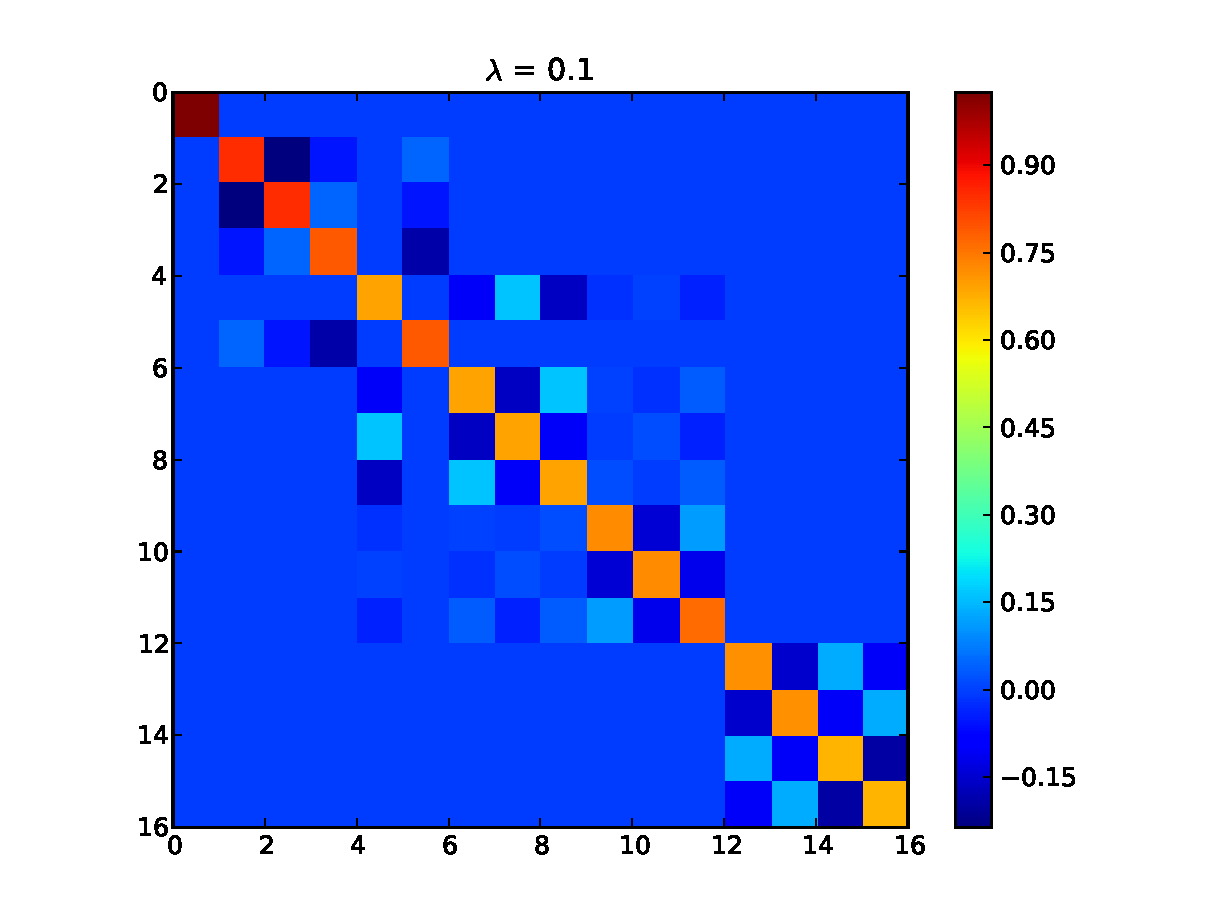
\includegraphics[scale=0.19]{../Code/Outputs/HOBasis/2_4/H01.pdf}}
\caption{Example with $N = 2$ particles and $R = 4$ shells}
\end{figure}
\end{frame}

\begin{frame}
\frametitle{Con: Time usage compared to simple exact diagonalization ...}
Example: $N = 6, R = 4$, on one processor
\begin{minipage}{0.6\linewidth}
\begin{table}
\begin{center}
\begin{tabular}{c c c}
\hline\hline
 $\lambda$ & $E_0$ & CPU time in $s$ \\
 \hline
 20.0 & \textbf{2}2.20366072 & 660 \\
% 17.0 & 22.18361918 & 1320 \\
 10.0 & \textbf{2}2.05448854 & 1756 \\
% 5.0 & \textbf{2}1.59433320 & 2387  \\
 3.0  & \textbf{2}0.99839817 & 2908  \\
 2.0  & \textbf{20}.57836962 & 3363 \\
 1.4  & \textbf{20.4}3153289 & 4608 \\
 1.0 & \textbf{20.416}04434 & 6813 \\
 0.8 & \textbf{20.41582}988 & 9126 \\
 0.6 & \textbf{20.41582765} & 14039 \\
\hline\hline
\end{tabular}
\end{center}
\caption{$E_0$ in units of $\hbar\omega = 2.84$ meV, from $\lambda = s^{-1/2}$ follows that $\left[\lambda\right] 
= \left[ E \right]$. The bold letters indicate correct digits.}
\end{table}
\end{minipage}
\begin{minipage}{0.35\linewidth}
\includegraphics[scale=0.21]{../Code/Outputs/HOBasis/6_4/time.pdf}
\vspace{1.5cm}
\end{minipage}

Time exact diagonalization (standard Armadillo method): $3s$  ($E_0 = 20.41582765$)\\
About {\color{red}{90\%}} of the time spent in {\color{red}{derivative function}}, increasing with dimension of $H$
\end{frame}

\section{Strategies to improve CPU time}
\begin{frame}
\frametitle{Problem: Fast increase of number basis states}

\begin{table}
\begin{center}
\begin{tabular}{c| c c c}
\hline
 $N$ & $R=3$ & $R = 5$ & $R = 7$ \\
 \hline
  2  & 8 & 29 & 72\\
  6  & 64 & 16451 & 594118\\
 12  & - & 1630953& 579968 \\ 
 \hline
\end{tabular}
\end{center}
\caption{Number $n$ of relevant basis states in M-scheme with constraint $M = M_s = 0$.}
\end{table}

Problem: Each call of the derivative function is of order  {\color{red}{$\mathcal{O}(n^3/2)$}} !!!\\
This explains the large CPU time ...
\end{frame}

\begin{frame}
\frametitle{Strategy 1: Reduce gradually size of the problem}
\begin{minipage}[b]{0.62\linewidth}
\begin{itemize}
\item Idea: After some integration, matrix elements far off the diagonal are \textbf{vanished} and will \textbf{stay zero}\\
\item $\Rightarrow$ those indices $i,j$ \textbf{not needed} any more when computing the derivatives

\begin{align*}
\frac{d V_{ij}}{ds } &= -(\epsilon_i - \epsilon_j)^2 V_{ij}(s) \\
&+ \sum\limits_k \left(\epsilon_i + \epsilon_j -2 \epsilon_k \right) V_{ik}(s) V_{kj}(s)
\end{align*}
\end{itemize}
\end{minipage}
\begin{minipage}[t]{0.35\linewidth}
\begin{center}
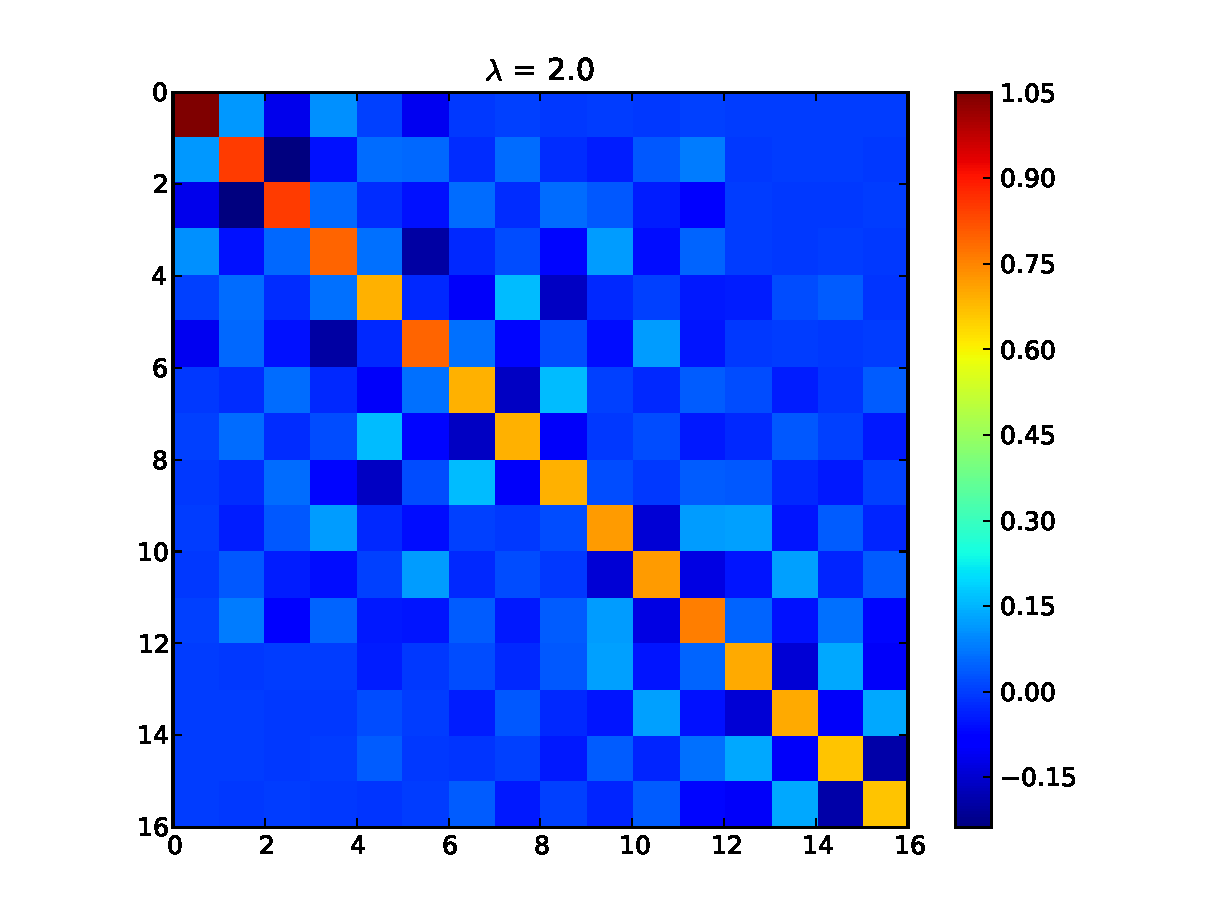
\includegraphics[scale=0.19]{../Code/Outputs/HOBasis/2_4/H2.pdf}
\end{center}
\end{minipage}

Therefore:
\begin{itemize}
\item  Save a {\color{red}{list}} with all elements $i,j$ that are needed for the derivative
\item In certain intervals, {\color{red}{delete those elements}} which are not needed any more (= where $V_{ij}(s)$ and $dV_{ij}(s)/ds$ are zero)
 \end{itemize}
\end{frame}

\begin{frame}
\frametitle{Strategy 1: Reduce gradually size of the problem}

%\begin{table}
%\begin{center}
%\begin{tabular}{c c c c}
%\hline\hline
%$\lambda$ & \# deleted elements & time [s] & time with all elements \\
%\hline 
% 20.0 & 7869 & 465& \\
%19.5 &7970 &740 & \\
%15.0 &7970 &1002 & \\
%10.0 &7970 &1258 & \\
%5.0 &7970 &1708 & \\
%2.0 & 7970 & 2411 & \\
%1.5 &7970 &1.5  &3047 & \\
%1.0 &7986 & 1 & 4852.039924 \\
% \\
% \hline\hline
%\end{tabular}
%\end{center}
%\caption{Time improvement by skipping matrix elements. System with $N = 6, R = 4$. Derivative function parallelized on 3 processors.}
%\end{table}

\begin{table}
\begin{center}
\subfigure[$N = 2, R = 8, n = 104$]{
\begin{tabular}{c |c c c c c }
\hline
$\lambda$      & 10.0 & 5.0 & 1.0 & 0.6& 0.4 \\
\hline skipped & 0 &0 &0 & 459 & 1943 \\
 \hline
\end{tabular}}

\subfigure[$N = 2, R = 9, n = 145$]{
\begin{tabular}{c |c c c c c c}
\hline
$\lambda$      & 10.0 & 5.0 & 1.0 & 0.8& 0.6 & 0.4  \\
\hline skipped & 0 &0 &12 & 393 & 1829 &  4921\\
 \hline
 \end{tabular}
}

\subfigure[$N = 6, R = 4, n = 1490$, Final time: 4162s vs. 4264s]{
\begin{tabular}{c |c c c c c c c }
\hline
$\lambda$      & 20.0 & 10.0 & 1.0 & 0.9& 0.8 & 0.7 & 0.6\\
\hline skipped & 7869 &8036 &8055 & 8578 & 11304 & 25072 & 68732\\
 \hline
\end{tabular}}


\end{center}
\caption{Reducing the size of the problem. Second line shows number of skipped matrix elements.}
\end{table}


\end{frame}


\begin{frame}
\frametitle{Strategy 2: Usage of optimized library routines}
Second attempt: Take benefit of optimized {\color{red}{matrix-matrix multiplication}} routines\\
Flow equation
\[
\frac{dV_s}{ds}  = \left[\eta_s, H_s\right]
\]
can be implemented as matrix-matrix multiplication with  $\eta_{ij}(s) = \left( \epsilon_i - \epsilon_j \right) V_{ij}(s)$ \\
and $H_{ij}(s) = \epsilon_i \delta_{ij} + V_{ij}(s)$

\textbf{Usage}: Blas routine for symmetric matrices ($V_{ij}(s) = V_{ji}(s)$)\\

\textbf{Result}: 
\begin{table}
\begin{center}
\begin{tabular}{c c c c}
\hline\hline
$N$ & $R$ & time [s] & time$_{\text{strategy1}}$ [s] \\
\hline 
2 & 9 & 15.78& 3.7 \\
2 & 10 & 26.9 & 10.8\\
 \hline\hline
\end{tabular}
\end{center}
\caption{Time comparison between both methods to reduce CPU time}
\end{table}
\textbf{Reasons} for more time:
\begin{itemize}
\item The matrix multiplication involves \textbf{more flops} than the pre-computed expression in Eq.(\ref{eq:flow})
%\item Blas returns \textbf{whole matrices}, actually just upper triangular part of $dV_{ij}(s)/ds$ needed
\item \textbf{No skipping} of elements possible as in the ansatz of the previous slides
\end{itemize}

\end{frame}


\section{Open questions}
\begin{frame}
\frametitle{Open questions}
Until now correct results, but exceedingly slow
\begin{itemize}
\item How to get a speedup? 
\item The problem lies in the $\mathcal{O}(n^3/2)$ flops each time the derivative function is called
\end{itemize}
For possibly larger systems
\begin{itemize}
\item The required memory to store the whole matrix explodes with number of particles/shells
\item Is there a smart way not to store the whole matrix (all interaction elements for the ODE solver)?
\end{itemize}


\end{frame}

\end{document}
